\begin{figure}[ht]
 \begin{center}
   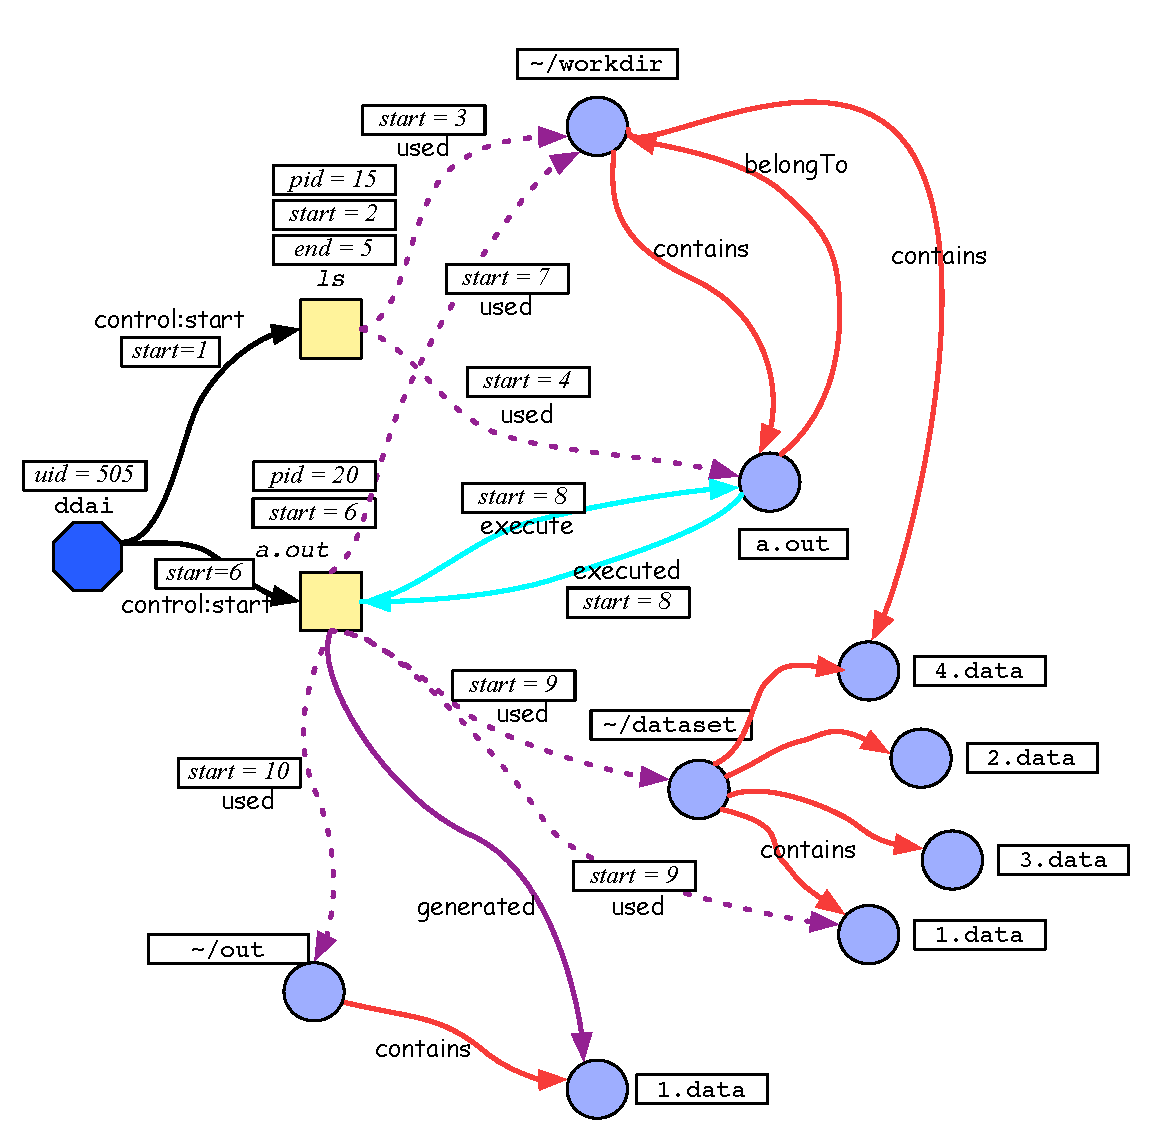
\includegraphics[width=3.2in]{images/exagraph.pdf}
   \caption{An example instance of metadata graph.}
   \label{exampleGraph}
 \end{center}
\end{figure}

Figure~\ref{exampleGraph} shows an example metadata graph, a user
named `ddai' with \textit{uid} $505$ executed two processes: \textit{ls} and
\textit{a.out} in order. First, he ran \textit{ls} in the `workdir' to
locate the executable file: `a.out'; after that, he started a process to
run this executable. The process will read data file under `dataset' with
name `1.data' and write data file under `out' with name `1.data' too. The
directory data object actually `contains' multiple other data objects.




\textit{gRMM} allows users to create their own relationships. The created relationships can be used to accelerate later query and
search. For example, given that a user `controls' a process, which will `use'
a data object, we can create a `visit' relationship between users and
data objects to record the visiting history of a user. This example is shown
in Fig.~\ref{nr}.

\begin{figure}[ht]
\begin{center}
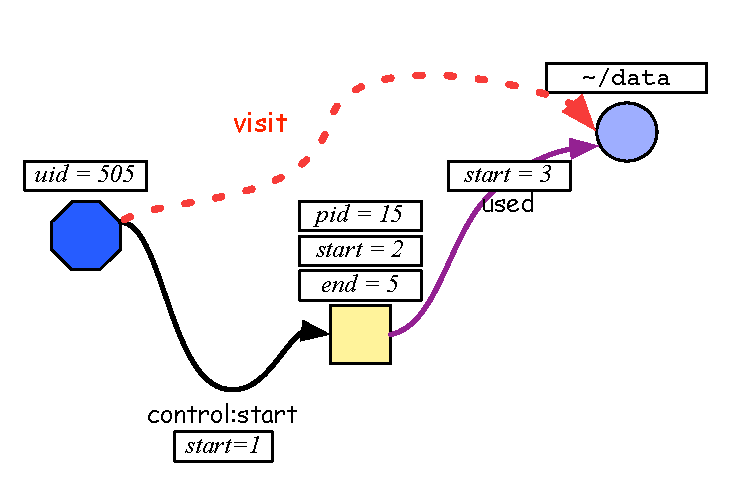
\includegraphics[width=3in]{images/newrelation.pdf}
\caption{An example of new relation named as \textit{visit}.}                                                                                  
\label{nr}
\end{center}
\end{figure}

There are two ways to create new relationship. The basic
way is to create an edge instance and connect it with
two existing vertice in the graph. This mechanism is mainly 
useful for relations that
cannot be inferred from existing relations. A simple example would be a
`recently created' relation between a data file and a user: whenever
a new file is created by a user, the application can add a specific
relation between them.

We also provide another way to create new relationships, called
\textit{combinations}. Users can submit a script that describes
how to combine existing relations to build a new one. For example,
generate a `visit' relation by combining `control' and `used'
relations as shown in Fig.~\ref{nr}. Submitting this script to 
\textit{gRMM} will trigger a distributed graph
task that results in the generation of new edges (relations).  The graph
will need to be submitted again to obtain updated results.
We will evaluate the practical implications of allowing users to submit
combination scripts to the system as well.  This feature may be restricted
to administrators for resource and security reasons.

In conclusion, the metadata graph model includes three basic predefined
entities and ten paired relations. Both the entities and relations contain unlimited user-defined properties which could be used as filter or search keywords.